
\mode<presentation> {

% The Beamer class comes with a number of default slide themes
% which change the colors and layouts of slides. Below this is a list
% of all the themes, uncomment each in turn to see what they look like.

%\usetheme{default}
%\usetheme{AnnArbor}
%\usetheme{Antibes}
%\usetheme{Bergen}
%\usetheme{Berkeley}
%\usetheme{Berlin}
%\usetheme{Boadilla}
%\usetheme{CambridgeUS}
% \usetheme{Copenhagen}
%\usetheme{Darmstadt}
%\usetheme{Dresden}
%\usetheme{Frankfurt}
%\usetheme{Goettingen}
%\usetheme{Hannover}
%\usetheme{Ilmenau}
%\usetheme{JuanLesPins}
%\usetheme{Luebeck}
%\usetheme{Madrid}
%\usetheme{Malmoe}
%\usetheme{Marburg}
%\usetheme{Montpellier}
\usetheme{PaloAlto}
%\usetheme{Pittsburgh}
%\usetheme{Rochester}
%\usetheme{Singapore}
%\usetheme{Szeged}
%\usetheme{Warsaw}

% As well as themes, the Beamer class has a number of color themes
% for any slide theme. Uncomment each of these in turn to see how it
% changes the colors of your current slide theme.

%\usecolortheme{albatross}
%\usecolortheme{beaver}
%\usecolortheme{beetle}
%\usecolortheme{crane}
%\usecolortheme{dolphin}
%\usecolortheme{dove}
%\usecolortheme{fly}
%\usecolortheme{lily}
%\usecolortheme{orchid}
%\usecolortheme{rose}
%\usecolortheme{seagull}
%\usecolortheme{seahorse}
%\usecolortheme{whale}
%\usecolortheme{wolverine}

%\setbeamertemplate{footline} % To remove the footer line in all slides uncomment this line
%\setbeamertemplate{footline}[page number] % To replace the footer line in all slides with a simple slide count uncomment this line

%\setbeamertemplate{navigation symbols}{} % To remove the navigation symbols from the bottom of all slides uncomment this line
}

\hypersetup{colorlinks=true,linkcolor=red,filecolor=magenta,urlcolor=cyan}
\usepackage{graphicx} % Allows including images
\usepackage{booktabs} % Allows the use of \toprule, \midrule and \bottomrule in tables
\usepackage{natbib}
\usepackage{apalike}
\usepackage{comment}
\usepackage{bm}
% \usepackage{enumitem}
% \setlist[itemize]{topsep=0pt,before=\leavevmode\vspace{-1.5em}}
% \setlist[description]{style=nextline}
\usepackage{amsthm}
\usepackage{media9}
% \usepackage{multimedia}
\usepackage{tikz}
\usetikzlibrary {positioning}
 \usetikzlibrary{overlay-beamer-styles}

\newtheorem{claim}{Claim}

\newenvironment{rowvector}
 {\bm{[}\begin{matrix}}
 {\end{matrix}\bm{]}}


%----------------------------------------------------------------------------------------
%	TITLE PAGE
%----------------------------------------------------------------------------------------

\title[LDS for Neuro]{Linear Dynamical Systems for Neuroscience} % The short title appears at the bottom of every slide, the full title is only on the title page

\author{Joaqu\'{i}n Rapela} % Your name
\institute[GCNU, UCL] % Your institution as it will appear on the bottom of every slide, may be shorthand to save space
{
Gatsby Computational Neuroscience Unit\\University College London % Your institution for the title page
}
\date{April 5, 2023} % Date, can be changed to a custom date

\AtBeginSection[]
  {
     \begin{frame}<beamer>
     \frametitle{Contents}
         \tableofcontents[currentsection,hideallsubsections]
     \end{frame}
  }

\begin{document}

\begin{frame}
\titlepage % Print the title page as the first slide
\end{frame}

\begin{frame}
\frametitle{Contents} % Table of contents slide, comment this block out to remove it
\tableofcontents % Throughout your presentation, if you choose to use \section{} and \subsection{} commands, these will automatically be printed on this slide as an overview of your presentation
\end{frame}

%----------------------------------------------------------------------------------------
%	PRESENTATION SLIDES
%----------------------------------------------------------------------------------------

\section{Introduction}

\begin{frame}
    \frametitle{Linear dynamical system lecture structure}

    \begin{enumerate}

        \item Introduction and motivation

        \item \textcolor{blue}{Inference}

            \begin{itemize}

                \item \textcolor{blue}{Kalman filter}

                \item \textcolor{blue}{Kalman smoother}

                \item \textcolor{blue}{Derviation of the Kalman filter equations}

            \end{itemize}

        \item Learning

            \begin{itemize}

                \item gradient ascent

                \item EM

            \end{itemize}

    \end{enumerate}
\end{frame}

\note[itemize] {

\item I will start the lecture with motivations about why LDSs are relevant to
    machine learning and highlight a few applications to biomedicine and
    healthcare. I will then cover inference and then learning in LDS.

\item In interest of time, today I will focus on the inference section.

}

\begin{frame}
    \frametitle{Linear dynamical systems}

    \begin{tikzpicture}[remember picture,overlay]
        \node[xshift=0cm,yshift=0cm] (ldsGraphicalModel) at (current page.center){%
                    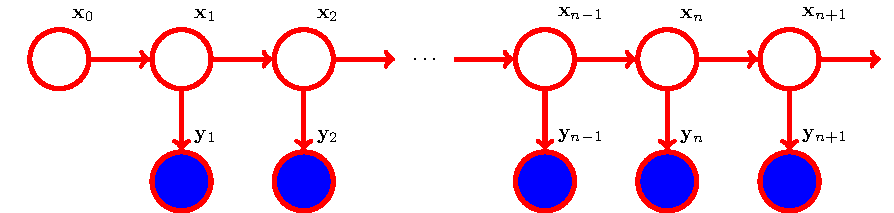
\includegraphics[width=3in]{figures/ldsGraphicalModel.pdf}};
            \node [below=of ldsGraphicalModel, visible on=<2->] {%
                    \includegraphics[width=.75in]{figures/radar.png}};
            \node [above=of ldsGraphicalModel, visible on=<3->] {%
                true planes positions, velocities and accelerations};
    \end{tikzpicture}

\end{frame}

\begin{frame}
    \frametitle{The linear dynamical system model}

    \begin{alignat*}{4}
        \mathbf{x}_n &= A \mathbf{x}_{n-1}+\mathbf{w}_n\quad && \mathbf{w}_n\sim
        N(\mathbf{w}_n|\mathbf{0}, Q)\quad && \mathbf{x}_n\in\mathbb{R}^M&&\\
        \mathbf{y}_n &= C \mathbf{x}_{n}+\mathbf{v}_n\quad && \mathbf{v}_n\sim
        N(\mathbf{v}_n|\mathbf{0}, R)\quad && \mathbf{y}_n\in\mathbb{R}^P&&\quad n=1\ldots N\\
        \mathbf{x}_0 &\sim N(\mathbf{w}_n|\mathbf{m}_0, V_0) && &&
    \end{alignat*}

    $\{\mathbf{x}_0, \mathbf{v}_n, \mathbf{w}_n\}_{n=1}^N$ uncorrelated

    \begin{figure}[h]
        \begin{center}
            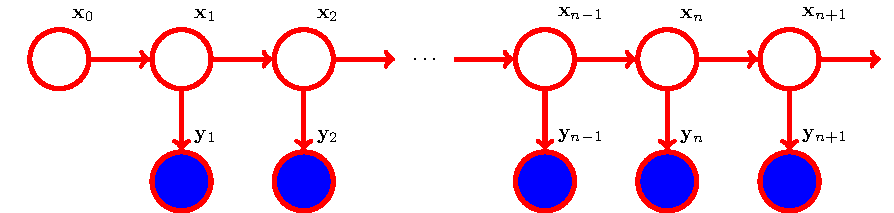
\includegraphics[width=4in]{figures/ldsGraphicalModel.pdf}
        \end{center}
    \end{figure}

    \textcolor{red}{$\{\mathbf{x}_0, \mathbf{x}_n, \mathbf{y}_n\}_{n=1}^N$ jointly normal}

    \note[itemize] {
        \scriptsize

        \item An observation $\mathbf{y}_n$ of a LDS is linear transformation
            of a latent variable $\mathbf{x}_n$ plus noise from a Gaussian
            distribution with mean and covariance R

        \item Latent variables follow an autoregressive model of order one.
            That is, the latent variable at time $n$ is a linear transformation
            of the latent at the pervious time plus Gaussian noise with mean 0
            and covariance Q.

        \item The initial state is a Gaussian random variable with mean $m_0$
            and covariance $V_0$.

        \item The initial state and all noise random variables are
            uncorrelated.

        \item Here is the graphical model for linear dynamical systems.

            This graphical model tell us that $x_n$ is dependent with
            $x_{n-1}$, as we see in the state equation, and that $y_n$ is
            dependent with $x_n$, as we see in the observation equation.

            Also, the D-separation property tell us two key independence
            properties of the joint distribution of states and observations.
            First, it show us that $x_{n+1}$ in indepedent of all previous x's,
            given $x_n$. This is call the Markov property. Second, it tell us
            that, given $x_n$, $y_n$ is independent of all previous and future
            observations.

            \normalsize
        }

\end{frame}

\begin{frame}
    \frametitle{Applications of linear dynamical systems in engineering}

    Apollo mission~\citep{mcGeeAndSchmidt85}, aircraft
    guidance~\citep{schmidtEtAl70}, GPS
    navigation~\citep{hofmannAndLichtenegger97}, weather
    forecasting~\citep{buehnerEtAl17}, etc.

    \vspace{.1in}

    \onslide<2->{
    Rudolf Emil Kalman received the 2008 Draper Prize from the National Academy
    of Engineering ``\textit{for the development and dissemination of the optimal
    digital technique (known as the Kalman filter) that is pervasively used to
    control a vast array of consumer, health, commercial, and defense
    products.}''
    }

    \note[itemize] {
        \scriptsize

        \item 

    }

\end{frame}

\begin{frame}
    \frametitle{Example application of linear dynamical systems in neuroscience}

    Decoding hand kinematics from motor cortex neural
    activity~\citep{wuEtAl06}.
%
    \textbf{Observation} ($y_n$): neural activity recorded from motor cortex of
    monkeys.
%
    \textbf{State} ($x_n$): hand position, velocity and acceleration.

    \begin{figure}[h]
        \begin{center}
            \includegraphics[width=4in]{figures/wuEtAl06_fig3a.png}
        \end{center}
    \end{figure}
    \hfill\citet{wuEtAl06}

\end{frame}

\begin{frame}
    \frametitle{SWC: inferring mouse kinematics from video recordings.}

    \begin{enumerate}
        \item \textbf{Observation} ($y_n$): noisy position estimates from
            DeepLabCut.
        \item \textbf{State} ($x_n$): mouse position, velocity and
            acceleration.
    \end{enumerate}

%     \begin{center}
%         \includemedia[
%             width=4.5cm,height=4.5cm,
%             activate=pageopen,
%             deactivate=onclick,
%             addresource=videos/FrameTop_2021-06-09T08-00-00_ss28_t60.avi,
%             flashvars={
%                 source=videos/FrameTop_2021-06-09T08-00-00_ss28_t60.avi
%                 &autoPlay=false
%             }
%             ]{}{VPlayer.swf}
%     \end{center}
    \hfill\tiny joint work with Foraging Working Group
\end{frame}

\begin{frame}
    \frametitle{SWC: inferring low-dimensional representations of neural population
    spiking activity.}

    \begin{enumerate}
        \item \textbf{Observation} ($y_n$): spike counts in 100~ms bins from neural population.
        \item \textbf{State} ($x_n$): low-dimensional representation of neural population spikes.
    \end{enumerate}
    \begin{columns}
    \column{0.5\textwidth}
        \href{http://www.gatsby.ucl.ac.uk/~rapela/mitra/reports/task_2019-02-06_21-36-35_preprocessing_2019_04_05_15_04_39_ks2/v1Shaft1/figures/92275409_smoothedStates.html}{\includegraphics[width=2.5in]{{figures/92275409_smoothedStates}.png}}
    \column{0.5\textwidth}
        \href{http://www.gatsby.ucl.ac.uk/~rapela/mitra/reports/task_2019-02-06_21-36-35_preprocessing_2019_04_05_15_04_39_ks2/v1Shaft1/figures/92275409_smoothedState1.html}{\includegraphics[width=2.5in]{{figures/92275409_smoothedState1}.png}} 

    \end{columns}
    \hfill\tiny joint work with Mitra Javadzadeh No

\end{frame}

\section{Design of a linear dynamical sytems for tracking}

\begin{frame}
    \frametitle{Discrete Wiener Process Acceleration (DWPA) model for tracking
    an object moving in 1D}

    \small

    \begin{alignat*}{3}
        \mathbf{x}_n &= A\mathbf{x}_{n-1} + \mathbf{w}_n && \quad \text{with} \quad\mathbf{w}_n\sim N(\mathbf{0}, Q) \quad \text{and} \quad\mathbf{x}_0\sim N(\mathbf{m}_0, V_0)\\
        y_n &= C\mathbf{x}_{n} + v_n                     && \quad \text{with} \quad v_n\sim N(0, \sigma^2)
    \end{alignat*}

    \begin{align*}
        \mathbf{x}_n&=\left[\xi[n],\dot{\xi}[n],\ddot{\xi}[n]\right]^\intercal\\
        A&=\begin{bmatrix}
            1 & T & T^2\\
            0 & 1 & T\\
            0 & 0 & 1
        \end{bmatrix}\\
        Q&=\gamma^2\begin{bmatrix}
            \frac{1}{4}T^4&\frac{1}{2}T^3&\frac{1}{2}T^2\\
            \frac{1}{2}T^3&T^2&T\\
            \frac{1}{2}T^2&T&1
        \end{bmatrix}\\
        C&=\begin{bmatrix}
            1 & 0 &0
        \end{bmatrix}
    \end{align*}

    \normalsize
    \note {
Starting with the equations of motion of a single particle, here I derive the
discrete Wiener process acceleration (DWPA) model~\citep[][Section 6.3.3
]{barShalomEtAl04}, a linear dynamical system for tracking an object moving in
one dimension. Then I extend this model for tracking an object moving in two
dimensions (Section~\ref{sec:dwpaModel2D}).
    }

\end{frame}

\begin{frame}
    \frametitle{Derivation of DWPA model for tracking}

    Consider the Taylor series expansion of the position as a function of time,
    $\xi(t)$, up to second order.

    \begin{align}
        \xi(t+T)&=\xi(t)+\dot{\xi}(t)T+\frac{\ddot{\xi}(t)}{2}T^2\label{eq:posTaylor2}
    \end{align}

    Approximations of the velocity and acceleration are derived from
    Eq.~\ref{eq:posTaylor2} by successive differentiation (with respect to
    $T$).

    \begin{align}
        \dot{\xi}(t+T)&=\dot{\xi}(t)+\ddot{\xi}(t)T\label{eq:velTaylor2}\\
        \ddot{\xi}(t+T)&=\ddot{\xi}(t)\label{eq:accTaylor2}
    \end{align}

\end{frame}

\begin{frame}
    \frametitle{Derivation of DWPA model for tracking}

    According to Eq.~\ref{eq:accTaylor2} the approximation of the acceleration,
    $\ddot{\xi}(t)$ is constant across all times. The DWPA model generalises
    this by replacing it with Eq.~\ref{eq:accDiscreteApprox}.

    \begin{align}
        \ddot{\xi}_a(t)=\ddot{\xi}(kT)+v(k)\quad t\in[kT,(k+1)T)\label{eq:accDiscreteApprox}
    \end{align}

    Replacing $\ddot{\xi}_a(t)$ by $\ddot{\xi}(t)$ in Eqs.~\ref{eq:posTaylor2},
    \ref{eq:velTaylor2} and~\ref{eq:accTaylor2} and discretizing we obtain the
    motion equations for the DWPA model.

    \begin{align}
        \xi(k+1)&=\xi(k)+\dot{\xi}(k)T+\frac{\ddot{\xi}(k)}{2}T^2+\frac{v(k)}{2}T^2\label{eq:posDWPA}\\
        \dot{\xi}(k+1)&=\dot{\xi}(k)+\ddot{\xi}(k)T+v(k)T\label{eq:velDWPA}\\
        \ddot{\xi}(k+1)&=\ddot{\xi}(k)+v(k)\label{eq:accDWPA}
    \end{align}

\end{frame}

\begin{frame}
    \frametitle{Derivation of DWPA model for tracking}

    Calling $x(k)=[\xi(k), \dot{\xi}(k), \ddot{\xi}(k)]^\intercal$,
    Eq.~\ref{eq:DWPAmodel} rewrites the previous
    equations in matrix form.

    \begin{align}
        x(k)&=\begin{bmatrix}
            1 & T & T^2\\
            0 & 1 & T\\
            0 & 0 & 1
            \end{bmatrix}
           x(k-1)+
           \begin{bmatrix}
               \frac{1}{2}T^2\\
               T\\
               1
           \end{bmatrix}
           v(k)\nonumber\\
           &=Ax(k-1)+\Gamma v(k)\nonumber\\
           &=Ax(k-1)+w(k)\label{eq:DWPAmodel}
    \end{align}

    We still need to find the covariance of $w(k)$.

\end{frame}

\begin{frame}
    \frametitle{Derivation of DWPA model for tracking}

    Because $v(k)\sim\mathcal{N}(0,\gamma^2)$ then $w(k)$ is also Gaussian with
    mean zero and covariance $Q$ (Eq.~\ref{eq:Q}).

    \begin{align}
        E\{w(k)\}&=\Gamma E\{v(k)\}=0\nonumber{}\\
        E\{w(k)w(k)^\intercal\}&=\Gamma E\{v(k)^2\}\Gamma^\intercal=\Gamma\gamma^2\Gamma^\intercal=\gamma^2\Gamma\Gamma^\intercal\nonumber\\
        &=\gamma^2\begin{bmatrix}
            \frac{1}{2}T^2\\
            T\\
            1
        \end{bmatrix}
        \raisebox{2.5ex}{
            $\begin{rowvector}\frac{1}{2}T^2, T, 1\end{rowvector}$
        }\nonumber\\
        &=\gamma^2\begin{bmatrix}
                    \frac{1}{4}T^4&\frac{1}{2}T^3&\frac{1}{2}T^2\\
                    \frac{1}{2}T^3&T^2&T\\
                    \frac{1}{2}T^2&T&1
        \end{bmatrix}=Q
        \label{eq:Q}
    \end{align}

\end{frame}

\begin{frame}
    \frametitle{Practical: sample from a DWPA model for tracking}

    \scriptsize
    \begin{align*}
        \mathbf{x}_n&=\left[\xi_{x}[n],\dot{\xi}_{x}[n],\ddot{\xi}_{x}[n],\xi_{y}[n],\dot{\xi}_{y}[n],\ddot{\xi}_{y}[n]\right]\\
        \mathbf{x}_n&=A\mathbf{x}_{n-1}+\mathbf{w}_n,\quad\mathbf{w}_n\sim\mathcal{N}(\mathbf{0},Q)\\
        \mathbf{y}_n&=\begin{bmatrix}
            1 & 0 & 0 & 0 & 0 &0\\
            0 & 0 & 0 & 1 & 0 &0\\
            \end{bmatrix}
            \mathbf{x}_n+\mathbf{v}_n,\quad\mathbf{v}_n\sim\mathcal{N}(\mathbf{0},R)\\
        \mathbf{x}_0&\sim\mathcal{N}(\mathbf{m}_0,V_0)
    \end{align*}
    \normalsize

    \begin{center}
        \href{}{\includegraphics[width=1.75in]{figures/simulated_pos.png}}
    \end{center}

    \hfill\href{https://joacorapela.github.io/lds_python/auto_examples/plotSimulatedTrajectoryDWPA.html\#sphx-glr-auto-examples-plotsimulatedtrajectorydwpa-py}{code}

\end{frame}

\note[itemize] {
\scriptsize
\item As a homework problem I will provide you the parameters of a LDS (e.g.,
    matrices A and C, noise covariance matrices Q and R, and the mean and
    covariance of the initial state). You will have to simulate states and
    observations from this LDS.

    The state equation of this LDS, models the motion equations of a particle.
    The state is six-dimensional. The first three components of this state
    represent the position, velocity and acceleration in the horizonal
    direction, and the last three components represent the position, velocity
    and acceleration in the vertical direction.

    The observations are two dimensional, and are noise-corrupted versions of
    the state horizonal and vertical positions.

    After simulating this LDS you will plot the vertical and horizontal
    position components of the state, and the observations.

    The figure shows my solution to this homework problem. The blue dots show
    the state position components and the black dots show the observations.

    We will next use the sampled observations to infer the state positions,
    velocities and accelerations.
\normalsize
}

\section{Inference}

\begin{frame}
    \frametitle{Inference in LDSs}

\begin{description}
    \item[Prediction]
        \begin{align}
            P(\mathbf{x}_n|\mathbf{y}_1,\ldots,\mathbf{y}_{n-1})=N(\mathbf{x}_n|\mathbf{x}_{n|n-1},P_{n|n-1})\nonumber
        \end{align}
    \item[Filtering]
        \begin{align}
            P(\mathbf{x}_n|\mathbf{y}_1,\ldots,\mathbf{y}_{n})=N(\mathbf{x}_n|\mathbf{x}_{n|n},P_{n|n})\nonumber
        \end{align}
    \item[Smoothing]
        \begin{align}
            P(\mathbf{x}_n|\mathbf{y}_1,\ldots,\mathbf{y}_{N})=N(\mathbf{x}_n|\mathbf{x}_{n|N},P_{n|N})\nonumber
        \end{align}
\end{description}

    \onslide<2->\textcolor{red}{{These conditional probabilities are Normal
    because $\{x_0, x_n, y_n\}_{n=1}^N$ are jointly normal.}}

\end{frame}

\note[itemize] {
\scriptsize
\item What does it mean to perform inference in LDSs? It means to learn
    properties of the state from the observations. The properties that we will
    learn are full probability distributions of the state at time $n$, $x_n$,
    given different sets of observations.

\item For prediction, we will learn the probability of the state at time $n$,
    given all previous observations. For filtering, we will learn the
    probability of the state at time $n$, given all previous observations plus
    the observation at time $n$. And for smoothing, we will learn the
    probability of the state at time $n$, given all previous and future
    observations.

\item Some notation. The mean of the prediction distribution is called
    $x_{n|n-1}$ because it is the mean of the probability of the state at time
    $n$ given all observations until time $n-1$.

    The mean of the filtering distribution is called $x_{n|n}$ because it is the
    mean of the probability of the state at time $n$ given all observations
    until time $n$.

    And the mean of the smoothing distribution is called $x_{n|N}$ because it
    is the mean of the probability of the state at time $n$ given all
    observations until time $N$.

\item Note that these conditional probabilities are Normal because all states
    and observations are jointly normal.
\normalsize
}

\subsection{Kalman filter}

\begin{frame}
    \frametitle{Kalman Filter}

The Kalman filtering algorithm estimates the prediction and filtering means and
    covariances: $x_{n|n-1}, P_{n|n-1}, x_{n|n}, .P_{n|n}$,

\scriptsize
\begin{alignat*}{2}
    \mathbf{x}_{0|0}&=\mathbf{m}_0&&\text{init filtered mean}\\
    P_{0|0}&=V_0&&\text{init filtered covariance}\\
    \mathbf{x}_{n+1|n}&=A\mathbf{x}_{n|n}\quad&&\text{prediction mean}\\
    P_{n+1|n}&=AP_{n|n}A^\intercal+Q\quad&&\text{prediction covariance}\\
    \mathbf{y}_{n|n-1}&=C\mathbf{x}_{n|n-1}\quad&&\text{predicted observation}\\
    \tilde{\mathbf{y}}_n&=\textcolor{red}{\mathbf{y}_n}-\mathbf{y}_{n|n-1}\quad&&\text{residual}\\
    S_n&=CP_{n|n-1}C^\intercal+R\quad&&\text{residual covariance}\\
    \mathbf{x}_{n|n}&=\mathbf{x}_{n|n-1}+K_n\tilde{\mathbf{y}}_n\quad&&\text{filtering mean}\\
    K_n&=P_{n|n-1}C^\intercal S_n^{-1}&&\text{Kalman gain}\\
    P_{n|n}&=(I_M-K_nC)P_{n|n-1}&&\text{filtering covariance}
\end{alignat*}
\normalsize

\end{frame}

\note[itemize]{
\scriptsize
\item The Kalman filtering algorithm estimates the prediction and filtering
    means and covariances: $x_{n|n-1}, P_{n|n-1}, x_{n|n}, .P_{n|n}$,

\item It initialized the filtering mean and covariances with those from the
    initial state.

\item Having calculated the filtering mean and convariances at time $n$, it
    calculates the prediction mean and covariances using these expression.

\item It then computes the predicted observation at time $n$ by linearly
    transforming the predicted state at time $n$.

\item Up to this point, the Kalman filter algorithm has not seen any
    observation. When observation $y_n$ arrives, the algorithm calculates the
    difference between this measurement and its prediction of it, which we call
    the residual, and caulates the covariance of this residual.

\item It then calculates the filtered mean by correcting the prediction mean
    with a a linea transformation of the residual.

    If the difference between the observation and its prediction was larger the
    predictive mean will be more corrected in generating the filering mean. The
    influence of the residual on the filtered mean is controlled by the Kalman
    gain matrix, whose expression appears below.

\item The last line gives the expression of the filtering covariance.
\normalsize

}

\begin{frame}
    \frametitle{Steps in the Kalman Filter}

% Inference of predicted and filtered means and covariances proceeds in a forward
% fashion, inferring the prediction and filtering distributions from the first to
% the last state, as shown in the next figure.

\scriptsize
% \begin{center}
    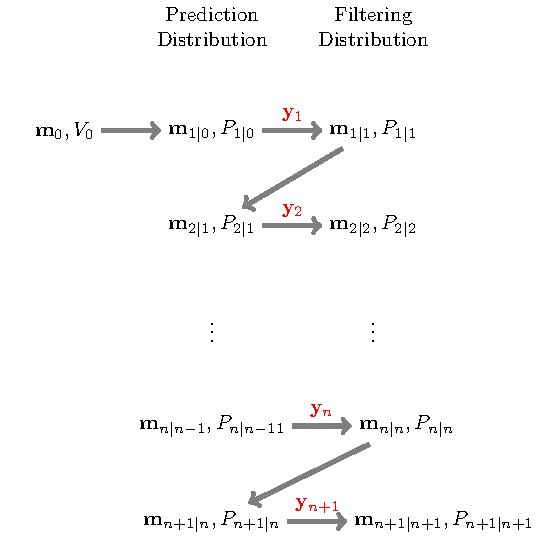
\includegraphics[width=3.0in]{figures/kfAlternations.pdf}
% \end{center}
\normalsize

    \onslide<2->{
        \textcolor{red}{forward, online}
    }

\end{frame}

\note[itemize]{
\item Here I illustrate the order of the calculations for the Kalman filter.

\item After initializing the mean and covariance of the filtering distribution,
    it calculates the mean and covariance of the predictive distribution.

\item When the first measurement arrives, it uses it to update the predictive
    mean and generate the filtered covariance, and it also generates the
    filtered covariance.

\item It repeats the preceding operations to calculate the predictiion and
    filtering distribution until the last sample time.

\item The Kalman filter operates in a foward fashing, starting with the
    caculation of the distribution at the first sample and finishing with the
    calculation for the last sample.

\item The Kalman filter algorithm can be used online. As soon as I receive an
    observation, I can compute the filtering distribution.
}

\begin{frame}
    \frametitle{Practical: infer filtered positions}

    \begin{center}
        \includegraphics[width=3in]{figures/filtered_pos.png}
    \end{center}
\end{frame}

\subsection{Kalman smoother}

\begin{frame}
    \frametitle{Kalman Smoother}

The Kalman smoother algorithm estimates the smoothed means and
    covariances: $x_{n|N}, P_{n|N}$.

\begin{alignat*}{2}
    x_{n|N}&=x_{n|n}+C_n(x_{n+1|N}-x_{n+1|n})\quad&&\text{smoothed mean}\\
    P_{n|N}&=P_{n|n}+C_n(P_{n+1|N}-P_{n+1|n})C_n^\intercal\quad&&\text{smoothed covariance}\\
    C_n&=P_{n|n}A^\intercal P_{n+1|n}^{-1}&&
\end{alignat*}

    \begin{itemize}

        \item The initial mean and covariances (i.e., $x_{N|N}, P_{N|N}$) are
            initialized from the last step of the Kalman filter.

        \item Smoothing proceeds in a \textcolor{red}{backward} fashion:

\scriptsize
    $x_{N|N}, P_{N|N}\rightarrow x_{N-1|N}, P_{N-1|N}\rightarrow x_{N-2|N},
    P_{N-2|N}\rightarrow\ldots\rightarrow  x_{1|N}, P_{1|N}$
\normalsize

        \item Smoothing can only be calculated \textcolor{red}{offline}.

    \end{itemize}

\end{frame}

\note[itemize]{

\item The Kalman smoother algorithm estimates the smoothed means and
    covariances: $x_{n|N}, P_{n|N}$.

\item The initial mean and covariances (i.e., $x_{N|N}, P_{N|N}$) are
    initialized from the last step of the Kalman filter.

\item The smoothed mean at time $n$ updates the filtered mean at time $n$ with
    a linear transformation of the difference between the smoothed mean at time
   $n+1$ and the prediction mean at time $n+1$.

\item The smoothing algorithm proceeds in a backward fashion. It starts with
    the calculation of the smoothed distribution at the last time and ends with
    this calculation at the first time.

\item Because all experimental samples are neede to compute the Kalman
    smoother, it can only be computed offline, after the experiment finished.

}

\begin{frame}
    \frametitle{Practical: infer the smoothed positions}

    \begin{center}
        \includegraphics[width=3in]{figures/smoothed_pos.png}
    \end{center}
\end{frame}

\begin{frame}
    \frametitle{Check that the state x position lies inside the 95\%
    confidence ellipse 95\% of the time}

    \begin{center}
        \includemedia[
            width=6cm,height=6cm,
            activate=pageopen,
            deactivate=onclick,
            addresource=videos/e1c-trueAndEstimatedStatesIn2D.mp4,
            flashvars={
                source=videos/e1c-trueAndEstimatedStatesIn2D.mp4
                &autoPlay=false
            }
            ]{}{VPlayer.swf}
    \end{center}

%     \begin{center}
% 
%         \movie{videos/e1c-trueAndEstimatedStatesIn2DFrame1.png}{videos/e1c-trueAndEstimatedStatesIn2D.mp4}
% 
%     \end{center}

\end{frame}

\section{Forecasting}

\section{Learning}

\subsection{Maximum likelihood by gradient ascent}

\subsection{Maximum likelihood by expectation maximization}

\section{Extensions}

\begin{frame}
\Huge{\centerline{Thanks}}
\end{frame}

\section{Appendix}

\subsection{Derivation of Kalman filter equations}

\begin{frame}
    \frametitle{Prediction mean}

    \scriptsize
\begin{claim}
    $\mathbf{x}_{n|n-1}=A\mathbf{x}_{n-1|n-1}$
    \label{claim:predictionMean}
\end{claim}

\begin{proof}
    \begin{align}
        \mathbf{x}_{n|n-1}&=E\{\mathbf{x}_n|\mathbf{y}_1,\ldots,\mathbf{y}_{n-1}\}\nonumber\\
                          &=E\{A\mathbf{x}_{n-1}+\mathbf{w}_n|\mathbf{y}_1,\ldots,\mathbf{y}_{n-1}\}\label{eq:c1l2}\\
                          &=AE\{\mathbf{x}_{n-1}|\mathbf{y}_ 1,\ldots,\mathbf{y}_{n-1}\}+E\{\mathbf{w}_n|\mathbf{y}_1,\ldots,\mathbf{y}_{n-1}\}\label{eq:c1l3}\\
                          &=A\mathbf{x}_{n-1|n-1}+E\{\mathbf{w}_n\}\label{eq:c1l4}\\
                          &=A\mathbf{x}_{n-1|n-1\label{eq:c1l5}}
    \end{align}
\end{proof}

Notes:

\begin{itemize}

    \item Eq.~\ref{eq:c1l2} arises from the state equation of the LDS model,
    \item Eq.~\ref{eq:c1l3} holds because the expectation distributes over sums
    \item Eq.~\ref{eq:c1l4} uses the definition of $\mathbf{x}_{n-1|n-1}$ and
        the fact that the state noise, $\mathbf{w}_n$, is independent of previous observations.
    \item Eq.~\ref{eq:c1l5} follows due to the zero mean of $\mathbf{w}_n$.

\end{itemize}
    \normalsize

\end{frame}

\begin{frame}
    \frametitle{Prediction covariance}
\scriptsize
\begin{claim}
    $P_{n|n-1}=AP_{n-1|n-1}A^\intercal+Q$
    \label{claim:predictionCov}
\end{claim}

\begin{proof}
    \begin{align}
        P_{n|n-1}=&\text{Cov}\{\mathbf{x}_n|\mathbf{y}_1,\ldots,\mathbf{y}_{n-1}\}\nonumber\\
                 =&\text{Cov}\{A\mathbf{x}_{n-1}+\mathbf{w}_n|\mathbf{y}_1,\ldots,\mathbf{y}_{n-1}\}\label{eq:c2l2}\\
                 =&\text{Cov}\{A\mathbf{x}_{n-1}|\mathbf{y}_1,\ldots,\mathbf{y}_{n-1}\}+\text{Cov}\{\mathbf{w}_n|\mathbf{y}_1,\ldots,\mathbf{y}_{n-1}\}\label{eq:c2l3}\\
                 =&A\ \text{Cov}\{\mathbf{x}_{n-1}|\mathbf{y}_1,\ldots,\mathbf{y}_{n-1}\}\ A^\intercal+\text{Cov}\{\mathbf{w}_n\}\label{eq:c2l4}\\
                 =&A\ P_{n-1|n-1}\ A^\intercal+Q\label{eq:c2l5}
    \end{align}
\end{proof}

Notes:

\begin{itemize}
    \item Eq.~\ref{eq:c2l2} used the state equation of the LDS model,
    \item Eq.~\ref{eq:c2l3} is true because $\mathbf{w}_n$ is indepedent from
        $\mathbf{x}_{n-1}$,
    \item Eq.~\ref{eq:c2l4} holds by the property
        $\text{Cov}\{A\mathbf{x}\}=A\ \text{Cov}\{\mathbf{x}\}' A^\intercal$ and
        because $\mathbf{w}_n$ is independent of previous observations.
    \item Eq.~\ref{eq:c2l5} applied the definitions of $P_{n-1|n-1}$ and $Q$.
\end{itemize}
\end{frame}

\begin{frame}
    \frametitle{Filtered mean and covariance}

    \scriptsize
    \begin{claim}
        $\mathbf{x}_{n|n}=\mathbf{x}_{n|n-1}+K_n\tilde{\mathbf{y}}_n$ and
        $P_{n|n}=(I-K_nC)P_{n|n-1}$.
        \label{claim:filteringMeanAndCov}
    \end{claim}

    \begin{proof}\renewcommand{\qedsymbol}{}

    Define the random variables
    $\mathbf{x}=\mathbf{x}_n|\mathbf{y}_1,\ldots,\mathbf{y}_{n-1}$ and
    $\mathbf{y}=\mathbf{y}_n|\mathbf{y}_1,\ldots,\mathbf{y}_{n-1}$. Then
    $\mathbf{x}|\mathbf{y}=\mathbf{x}_n|\mathbf{y}_1,\ldots,\mathbf{y}_n$ and
    the mean and covariance that we want to find, $\mathbf{x}_{n|n}$ and
    $P_{n|n}$, are those of $\mathbf{x}|\mathbf{y}$.  Thus, we want to compute
    the mean, $\mu_{\mathbf{x}|\mathbf{y}}=\mathbf{x}_{n|n}$, and covariance,
    $\Sigma_{\mathbf{x}|\mathbf{y}}=P_{n|n}$, of $\mathbf{x}|\mathbf{y}$.

    Because $\mathbf{x}_n$ and $\mathbf{y}_n$ are jointly Gaussian, then
    $\mathbf{x}$ and $\mathbf{y}$ are also jointly Gaussian. Then, $\mu_{\mathbf{x}|\mathbf{y}}$
    and $\Sigma_{\mathbf{x}|\mathbf{y}}$ are \citep[][Chapter 2]{bishop06}

    \begin{align}
        \mu_{\mathbf{x}|\mathbf{y}}&=\mu_{\mathbf{x}} +
        \Sigma_{\mathbf{x}\mathbf{y}}\Sigma_{\mathbf{y}\mathbf{y}}^{-1}(\mathbf{y}_n-\mu_{\mathbf{y}})\label{eq:muxgy}\\
        \Sigma_{\mathbf{x}|\mathbf{y}}&=\Sigma_{\mathbf{x}\mathbf{x}}-\Sigma_{\mathbf{x}\mathbf{y}}\Sigma_{\mathbf{y}\mathbf{y}}^{-1}\Sigma_{\mathbf{y}\mathbf{x}}\label{eq:sigmaxgy}
    \end{align}

    Thus, to compute $\mu_{\mathbf{x}|\mathbf{y}}$ and $\Sigma_{\mathbf{x}|\mathbf{y}}$ we need to calculate
    $\mu_{\mathbf{x}}$, $\mu_{\mathbf{y}}$, $\Sigma_{\mathbf{x}\mathbf{x}}$, $\Sigma_{\mathbf{x}\mathbf{y}}$ and $\Sigma_{\mathbf{y}\mathbf{y}}$.

        % \alt<3>{\qedhere}{\phantom\qedhere}

    \end{proof}

    \normalsize
\end{frame}

\begin{frame}
    \frametitle{Filtered mean and covariance (cont)}
    \scriptsize

    \begin{proof}\renewcommand{\qedsymbol}{}
    \begin{align}
        \mu_{\mathbf{x}}&=E\{\mathbf{x}\}=E\{\mathbf{x}_n|\mathbf{y}_1,\ldots\mathbf{y}_{n-1}\}=\mathbf{x}_{n|n-1}\label{eq:mux}\\
        \mu_{\mathbf{y}}&=E\{\mathbf{y}\}=E\{\mathbf{y}_n|\mathbf{y}_1,\ldots\mathbf{y}_{n-1}\}=E\{C\mathbf{x}_n+\mathbf{v}_n|\mathbf{y}_1,\ldots\mathbf{y}_{n-1}\}=\nonumber\\
             &=CE\{\mathbf{x}_n|\mathbf{y}_1,\ldots\mathbf{y}_{n-1}\}+E\{\mathbf{v}_n|\mathbf{y}_1,\ldots\mathbf{y}_{n-1}\}=C\mathbf{x}_{n|n-1}+E\{\mathbf{v}_n\}\nonumber\\
             &=C\mathbf{x}_{n|n-1}=\mathbf{y}_{n|n-1}\label{eq:muy}
    \end{align}
        % \alt<3>{\qedhere}{\phantom\qedhere}
    \end{proof}

    Notes:

    \begin{itemize}
        \item The fifth equality in Eq.~\ref{eq:muy} uses the definition
            of $\mathbf{x}_{n|n-1}$ and the fact that $\mathbf{v}_n$ is
            independent of previous observations.

        \item The last equality in Eq.~\ref{eq:muy} holds because the mean of
            $\mathbf{v}_n$ is zero.
    \end{itemize}

    \normalsize
\end{frame}

\begin{frame}
    \frametitle{Filtered mean and covariance (cont)}
    \scriptsize

    \begin{proof}\renewcommand{\qedsymbol}{}
    \begin{align}
        \Sigma_{\mathbf{y}\mathbf{y}}&=\text{Cov}(\mathbf{y}_n|\mathbf{y}_1,\ldots,\mathbf{y}_{n-1})\nonumber\\
                                     &=\text{Cov}(C\mathbf{x}_n+\mathbf{v}_n|\mathbf{y}_1,\ldots,\mathbf{y}_{n-1})\nonumber\\
                                     &=\text{Cov}(C\mathbf{x}_n|\mathbf{y}_1,\ldots,\mathbf{y}_{n-1})+\text{Cov}(\mathbf{v}_n|\mathbf{y}_1,\ldots,\mathbf{y}_{n-1})\nonumber\\
                                     &=C\ \text{Cov}(\mathbf{x}_n|\mathbf{y}_1,\ldots,\mathbf{y}_{n-1})\ C^\intercal+\text{Cov}(\mathbf{v}_n)\label{eq:c3Sigmayyl4}\\
                                     &=CP_{n|n-1}C^\intercal+R\label{eq:sigmayy}
    \end{align}
    \end{proof}

Notes:

\begin{itemize}

    \item As in Eq.~\ref{eq:c2l3}, Eq.~\ref{eq:c3Sigmayyl4} holds by the
        property
        $\text{Cov}\{A\mathbf{x}\}=A\ \text{Cov}\{\mathbf{x}\}\ A^\intercal$ and
        because $\mathbf{v}_n$ is independent of previous observations.

\end{itemize}
\end{frame}

\begin{frame}
    \frametitle{Filtered mean and covariance (cont)}
    \scriptsize

    \begin{proof}\renewcommand{\qedsymbol}{}
    \begin{align}
        \Sigma_{\mathbf{x}\mathbf{y}}&=\text{cCov}(\mathbf{x}_n,\mathbf{y}_n|\mathbf{y}_1,\ldots,\mathbf{y}_{n-1})\nonumber\\
                                     &=\text{cCov}(\mathbf{x}_n,C\mathbf{x}_n+\mathbf{v}_n|\mathbf{y}_1,\ldots,\mathbf{y}_{n-1})\nonumber\\
                                     &=\text{cCov}(\mathbf{x}_n,C\mathbf{x}_n|\mathbf{y}_1,\ldots,\mathbf{y}_{n-1})+\text{cCov}(\mathbf{x}_n,\mathbf{v}_n|\mathbf{y}_1,\ldots,\mathbf{y}_{n-1})\label{eq:c3Sigmaxyl3}\\
                                     &=\text{Cov}(\mathbf{x}_n|\mathbf{y}_1,\ldots,\mathbf{y}_{n-1})C^\intercal+0\label{eq:c3Sigmaxyl4}\\
                                     &=P_{n|n-1}C^\intercal\label{eq:sigmaxy}
    \end{align}
    \end{proof}

    Notes:

    \begin{itemize}
        \item the first term in Eq.~\ref{eq:c3Sigmaxyl4} arises from the first
            term of Eq.~\ref{eq:c3Sigmaxyl3} since

            \begin{align*}
                \text{cCov}(\mathbf{x}_n,C\mathbf{x}_n|\mathbf{y}_1,\ldots,\mathbf{y}_{n-1})&=E\{(\mathbf{x}_n-\mu_\mathbf{x})(C\mathbf{x}_n-C\mu_{\mathbf{x}})^\intercal|\mathbf{y}_1,\ldots,\mathbf{y}_{n-1}\}\\
                                                                                            &=E\{(\mathbf{x}_n-\mu_\mathbf{x})(\mathbf{x}_n-\mu_{\mathbf{x}})^\intercal C^\intercal|\mathbf{y}_1,\ldots,\mathbf{y}_{n-1}\}\\
                                                                                            &=E\{(\mathbf{x}_n-\mu_\mathbf{x})(\mathbf{x}_n-\mu_{\mathbf{x}})^\intercal|\mathbf{y}_1,\ldots,\mathbf{y}_{n-1}\}C^\intercal\\
                                                                                            &=\text{Cov}(\mathbf{x}_n|\mathbf{y}_1,\ldots,\mathbf{y}_{n-1})C^\intercal
            \end{align*}

    \end{itemize}
\end{frame}

\begin{frame}
    \frametitle{Filtered mean and covariance (cont)}
    \scriptsize

    \begin{proof}\renewcommand{\qedsymbol}{}
    \begin{align}
        \Sigma_{\mathbf{x}\mathbf{y}}&=\text{cCov}(\mathbf{x}_n,\mathbf{y}_n|\mathbf{y}_1,\ldots,\mathbf{y}_{n-1})\nonumber\\
                                     &=\text{cCov}(\mathbf{x}_n,C\mathbf{x}_n+\mathbf{v}_n|\mathbf{y}_1,\ldots,\mathbf{y}_{n-1})\nonumber\\
                                     &=\text{cCov}(\mathbf{x}_n,C\mathbf{x}_n|\mathbf{y}_1,\ldots,\mathbf{y}_{n-1})+\text{cCov}(\mathbf{x}_n,\mathbf{v}_n|\mathbf{y}_1,\ldots,\mathbf{y}_{n-1})\label{eq:c3Sigmaxyl3}\\
                                     &=\text{Cov}(\mathbf{x}_n|\mathbf{y}_1,\ldots,\mathbf{y}_{n-1})C^\intercal+0\label{eq:c3Sigmaxyl4}\\
                                     &=P_{n|n-1}C^\intercal\label{eq:sigmaxy}\\
        \Sigma_{\mathbf{x}\mathbf{x}}&=\text{Cov}(\mathbf{x}_n|\mathbf{y}_1,\ldots,\mathbf{y}_{n-1})=P_{n|n-1}\label{eq:sigmaxx}
    \end{align}
    \end{proof}

    Notes:

    \begin{itemize}
        \item the first term in Eq.~\ref{eq:c3Sigmaxyl4} arises from the first
            term of Eq.~\ref{eq:c3Sigmaxyl3} since

            \begin{align*}
                \text{cCov}(\mathbf{x}_n,C\mathbf{x}_n|\mathbf{y}_1,\ldots,\mathbf{y}_{n-1})&=E\{(\mathbf{x}_n-\mu_\mathbf{x})(C\mathbf{x}_n-C\mu_{\mathbf{x}})^\intercal|\mathbf{y}_1,\ldots,\mathbf{y}_{n-1}\}\\
                                                                                            &=E\{(\mathbf{x}_n-\mu_\mathbf{x})(\mathbf{x}_n-\mu_{\mathbf{x}})^\intercal C^\intercal|\mathbf{y}_1,\ldots,\mathbf{y}_{n-1}\}\\
                                                                                            &=E\{(\mathbf{x}_n-\mu_\mathbf{x})(\mathbf{x}_n-\mu_{\mathbf{x}})^\intercal|\mathbf{y}_1,\ldots,\mathbf{y}_{n-1}\}C^\intercal\\
                                                                                            &=\text{Cov}(\mathbf{x}_n|\mathbf{y}_1,\ldots,\mathbf{y}_{n-1})C^\intercal
            \end{align*}

    \end{itemize}
\end{frame}

\begin{comment}
\end{comment}

\begin{frame}
    \frametitle{Filtered mean and covariance (cont)}
    \scriptsize

    \begin{itemize}

        \item the second term in Eq.~\ref{eq:c3Sigmaxyl4} arises from the
            second
            term of Eq.~\ref{eq:c3Sigmaxyl3} since

            \begin{align*}
                \text{cCov}(\mathbf{x}_n,\mathbf{v}_n|\mathbf{y}_1,\ldots,\mathbf{y}_{n-1})&=E\{(\mathbf{x}_n-\mathbf{x}_{n|n-1})\mathbf{v}_n|\mathbf{y}_1,\ldots,\mathbf{y}_{n-1}\}\\
                                                                                           &=E\{(\mathbf{x}_n-\mathbf{x}_{n|n-1})|\mathbf{y}_1,\ldots,\mathbf{y}_{n-1}\}E\{\mathbf{v}_n|\mathbf{y}_1,\ldots,\mathbf{y}_{n-1}\}\\
                                                                                           &=E\{(\mathbf{x}_n-\mathbf{x}_{n|n-1})|\mathbf{y}_1,\ldots,\mathbf{y}_{n-1}\}E\{\mathbf{v}_n\}\\
                                                                                           &=E\{(\mathbf{x}_n-\mathbf{x}_{n|n-1})|\mathbf{y}_1,\ldots,\mathbf{y}_{n-1}\}0\\
                                                                                           &=0
            \end{align*}

            the second line follows from the first one because $\mathbf{v}_n$
            is independent of $\mathbf{x}_n$, and the third line follows from
            the second one because $\mathbf{v}_n$ is indepednent of previous
            observations.

    \end{itemize}
    \normalsize
\end{frame}

\begin{frame}
    \frametitle{Filtered mean and covariance (cont)}
    \scriptsize

    \begin{proof}
    Having calculated $\mu_{\mathbf{x}}$, $\mu_{\mathbf{y}}$,
    $\Sigma_{\mathbf{x}\mathbf{x}}$, $\Sigma_{\mathbf{x}\mathbf{y}}$ and
    $\Sigma_{\mathbf{y}\mathbf{y}}$ we now use Eqs.~\ref{eq:muxgy},
    \ref{eq:sigmaxgy}, \ref{eq:mux},  \ref{eq:muy},  \ref{eq:sigmayy},
    \ref{eq:sigmaxy}, and \ref{eq:sigmaxx} to  
    obtain $\mathbf{x}_{n|n}$ and $P_{n|n}$.

    \begin{align*}
        \mathbf{x}_{n|n}=\mu_{\mathbf{x}|\mathbf{y}}&=\mu_{\mathbf{x}} + \Sigma_{\mathbf{x}\mathbf{y}}\Sigma_{\mathbf{y}\mathbf{y}}^{-1}(\mathbf{y}_n-\mu_{\mathbf{y}})\\
                                                    &=\mathbf{x}_{n|n-1}+P_{n|n-1}C^\intercal S_n^{-1}(\mathbf{y}_n-\mathbf{y}_{n|n-1})\\
                                                    &=\mathbf{x}_{n|n-1}+K_n\tilde{\mathbf{y}_n}\\
        P_{n|n}=\Sigma_{\mathbf{x}|\mathbf{y}}&=\Sigma_{\mathbf{x}\mathbf{x}}-\Sigma_{\mathbf{x}\mathbf{y}}\Sigma_{\mathbf{y}\mathbf{y}}^{-1}\Sigma_{\mathbf{y}\mathbf{x}}\\
                                              &=P_{n|n-1}-P_{n|n-1}C^\intercal S_n^{-1}CP_{n|n-1}\\
                                              &=(I-P_{n|n-1}C^\intercal S_n^{-1}C)P_{n|n-1}\\
                                              &=(I-K_nC)P_{n|n-1}
    \end{align*}
    \end{proof}
    \normalsize
\end{frame}

\begin{frame}
\frametitle{References}
\tiny{
\bibliographystyle{apalike}
\bibliography{machinelearning,epilepsy,stats,gaussianProcesses,eeg,latentsVariablesModels,linearDynamicalSystems}
}
\end{frame}

%----------------------------------------------------------------------------------------

\end{document} 
%------------------------------------------------
